\documentclass[tikz]{standalone}

\pagestyle{empty}

\usepackage{amsmath}
\usepackage{tikz}
\usepackage{graphicx}
\usetikzlibrary{positioning,calc,fit,decorations.pathreplacing,arrows,positioning,backgrounds}

% Font settings:
\renewcommand{\familydefault}{\sfdefault}
\usepackage{pxfonts}
\newcommand{\figf}{\sffamily\bfseries\small} %Defines the font used for the labelling of figure panels.


% Color settings:
%\definecolor{hivc}{cmyk}{0,0.80,0.83,0.13}                %\definecolor{hivc}{HTML}{DE2D26}
\definecolor{hivc}{RGB}{24,116,205}
\definecolor{selfc}{cmyk}{0,0,0,0.6}                      %\colorlet{selfc}{gray!80!white}
\definecolor{Rblue}{RGB}{100,149,237}



%__________________________________________________________________________
%__________________________________________________________________________
%%----BEGINNING OF DOCUMENT
%__________________________________________________________________________
%__________________________________________________________________________

\begin{document}
\scriptsize

%---------------------------------FIGURE 6: PEPTIDE SELECTION---------------------------------


\begin{tikzpicture}[anchor=north west]
\clip (0,0.3) rectangle (12,-6.5);


\begin{scope}

  \node[anchor=north west,align=left] (he) at (0.2,-0.3) {highly\\exchangeable};
  \draw[-stealth] (0.95,-0.95) -- +(0.2,-0.2);

  \node[anchor=north east,align=right] at (3.3, 0.05) {slightly\\exchangeable};
  \draw[-stealth] (2.80,-0.6) -- +(-0.2, -0.2);

  \node[anchor=north east] at (3.3,-2.53) {not exchangeable};
  \draw[-stealth] (3.05,-2.53) -- +(-0.2,0.2);
  
  \node[scale=0.3] at (0.8,-0.7) {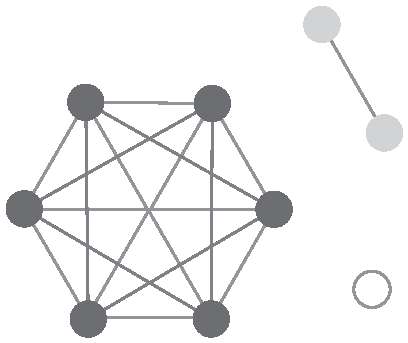
\includegraphics{../cartoons/clusters.pdf}};
  \node at (0,0.3) {\figf A};


\end{scope}

\begin{scope}[xshift=4.1cm]
	\node[scale=0.75] at (0,0) {\includegraphics{../plots/F6panelB.pdf}};
	\filldraw[white] (0.6,-2.5) rectangle (4.1,-2.9);
	\node[anchor=north] at (2.5, -2.5) {x1000 training peptides};

	\node[anchor = north west] (R) at (1.9,-0.9) {random};
	\draw[-stealth] (R.west) -- +(-0.2,0.2);
	\node[anchor = north west] (O) at (1.18,-0.1) {optimal};
	\draw[-stealth] (1.28,-0.43) -- +(0.2,-0.2);
	\node at (0,0.3) {\figf B};
\end{scope}

\begin{scope}[xshift=8.1cm]
  \node[scale=0.75] at (0,0) {\includegraphics{../plots/F6panelC.pdf}};
  \node at (0,0.3) {\figf C};
\end{scope}



\begin{scope}[xshift=0cm,yshift=-3.1cm]
  \begin{scope}[xshift=0cm]
  \node[scale=0.75] at (0,-0.3) {\includegraphics{../plots/F6panelD.pdf}};
  \filldraw[white] (0.6,-2.8) rectangle (4.2,-3.2);
  \node[anchor=north] at (2.6, -2.8) {x1000 training peptides};
  \node[anchor=north west](O) at (3.0,-0.55) {optimal};
  \node[anchor=north west](R) at (3.0,-1.63){random};
  \end{scope}
  \node at (0,0) {\figf  D};

\end{scope}

\begin{scope}[yshift=-3.1cm,xshift=4.1cm]
  \node[scale=0.75] at (0,-0.3) {\includegraphics{../plots/F6panelE.pdf}};
  \node at (0,0) {\figf  E};
\end{scope}


\end{tikzpicture}






\end{document}